\chapter{Thermodynamics}


\subsection{thermal physics basics}


\subsection{temperature scales}\label{s-temp-scale}

\begin{marginfigure}
	\centering
	\vspace*{-2.7cm}
	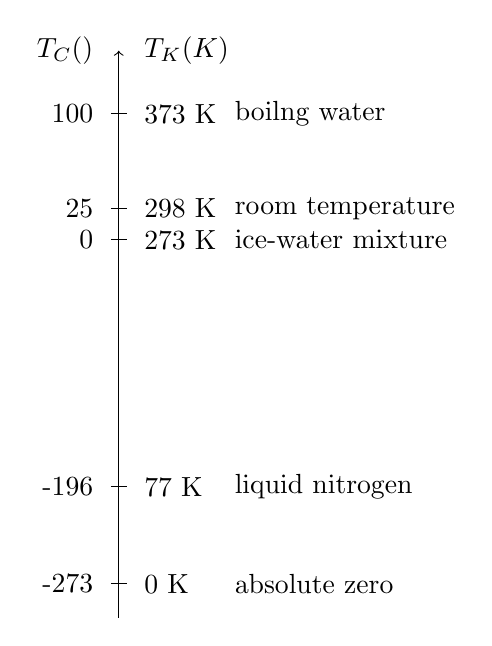
\begin{tikzpicture}[yscale=1.6]
	\draw[->] (0,-3) -- (0,1.50);
	\foreach \temp in {-2.73,-1.96,0,0.25,1.00} \draw (-0.1,\temp) --++ (0.2,0);
	\node[left] at (-0.2,1.5) {$T_C(\OC)$};
	\node[right] at (0.2,1.5) {$T_K(\text{K})$};
	\node[left] at (-0.2,-2.73) {-273\OC};
	\node[left] at (-0.2,-1.96) {-196\OC};
	\node[left] at (-0.2,-0) {0\OC};
	\node[left] at (-0.2,0.25) {25\OC};
	\node[left] at (-0.2,1) {100\OC};
	\node[right] at (0.2,-2.73) {0 K};
	\node[right] at (0.2,-1.96) {77 K};
	\node[right] at (0.2,-0) {273 K};
	\node[right] at (0.2,0.25) {298 K};
	\node[right] at (0.2,1) {373 K};
	\node[right] at (1.35,-2.73) {absolute zero};
	\node[right] at (1.35,-1.96) {liquid nitrogen};
	\node[right] at (1.35,0) {ice-water mixture};
	\node[right] at (1.35,0.25) {room temperature};
	\node[right] at (1.35,1.00) {boilng water};
	\end{tikzpicture}
	\vspace*{-30pt}
\end{marginfigure}

\cmt Celsius scale (unit: \OC)

0$^\circ$C defined as temperature of ice-water mixture

100$^\circ$C defined as temperature of boiling water

\cmt Kelvin scale (unit: K)

0 K (\emph{absolute zero}) is lowest temperature possible

\cmt conversion rule: $T_K (\text{K}) \text{ } \autorightleftharpoons{\footnotesize -273}{\footnotesize +273} \text{ } T_C (\OC)$

\cmt change of 1$^\circ$C equals change of 1 K


\subsection{kinetic theory of matter}

there are three common states of matter: solid, liquid and gas

they have very different physical properties (density, compressibility, fluidity, etc.)

but deep down, they are all composed of a large number of small molecules

in the \keypoint{kinetic theory of matter}, we look at microscopic behaviour at molecular level (arrangement, motion, intermolecular forces, separation, etc.)

\emph{microscopic} behaviour of molecules cause differences in \emph{macroscopic} properties of matter

\begin{compactitem}
	\item[--] solid: molecules close together, tightly bonded, vibrate about their positions
	
	\item[--] liquid: molecules quite close together, vibrate but has some freedom to move about
	
	\item[--] gas: molecules widely separated, free from neighbours, move rapidly
\end{compactitem}

\subsection{specific latent heat}

it requires heat energy to \emph{melt} a solid or \emph{boil} a liquid

melting and boiling usually occur at a fixed temperature

thermal energy to cause the change of state at a constant temperature is called \emph{latent heat}

amount of latent heat needed depends on mass of substance: $\boxed{Q=Lm}$

\begin{ilight}
	we define \keypoint{specific latent heat}\index{specific latent heat} ($L$) as the thermal energy required to change the state of \emph{unit} mass of substance with no change in temperature is called 
\end{ilight}



\cmt unit of specific latent heat: $[L] = \text{J}\cdot\text{kg}^{-1}$

\cmt specific latent heat is an \emph{intensive} property

i.e., $L$ does not depend on size or shape of sample, $L$ depends on type of substance only 
	
\cmt for melting, $L$ is called \emph{specific latent heat of fusion}
	
for boiling, $L$ is called \emph{specific latent heat of vaporisation}
	
\cmt latent heat is related to breaking bonds and increasing intermolecular separation
	
vaporisation requires larger increase in particle separation than fusion
	
for a given substance, $L_\text{vapour}>L_\text{fuse}$


\example{A 3.0 kW electric kettle contains 0.5 kg of water already at its boiling point. Neglecting heat losses, determine how long it takes to boil dry. ($L_\text{water} = 2.26 \times 10^6 \text{ J kg}^{-1}$)}
	
\sol heat required: $Q=mL = 0.50 \times 2.26 \times 10^6 = 1.13 \times 10^6 \text{ J}$
	
time needed: $t=\frac{Q}{P} = \frac{1.13 \times 10^6}{3.0\times 10^3} \approx 380 \text{ s} \approx 6.3 \text{ min}$ \eoe
 
\example{A student measures specific latent heat of fusion for ice. He uses an electric heater to melt ice but the insulation is not perfect. The experiment is carried out twice, with the heater operating at different powers. Use the data table to calculate specific latent heat of fusion.}

\begin{center}
	\begin{tabular}{|C{1.6cm}|C{2cm}|c|c|}
		\hline  & Power (W) & time interval (min) & mass of ice melted (g) \\ 
		\hline test 1 & 60 & 3.0 & 40.4 \\ 
		\hline test 2 & 90 & 3.0 & 56.6 \\ 
		\hline 
	\end{tabular} 
\end{center}

\sol there exists heat gain from surroundings, so effective power $P_\text{eff}=P_\text{heater}+P_\text{sur}$

heat energy to melt ice: $Q = mL = (P_\text{heater}+P_\text{sur}) t$
\begin{equation*}
	\left\{ \begin{array}{l}
		40.4 \times L = (60+P_\text{sur})\times3.0\times60 \\
		56.6 \times L = (90+P_\text{sur})\times3.0\times60 
	\end{array}\right.
	\RA \left\{ \begin{array}{l}
	L \approx 333 \text{ J g}^{-1} \\
	P_\text{sur} \approx 14.8 \text{ W} \end{array}\right. 
\end{equation*}

\eqyskip

\question{A student designs an experiment to determine the specific latent heat of fusion $L$ of ice. Some ice at $0\OC$ is heated with an electric heater. The experiment is carried out twice and the following data are obtained.
	
\begin{center}
	\begin{tabular}{|c|c|c|c|}
		\hline  & energy supply from heater (J) & time interval (min) & mass of ice melted (g) \\ 
		\hline heater off & 0 & 10.0 & 14.3 \\ 
		\hline heater on & 21000 & 5.0 & 70.0 \\ 
		\hline 
	\end{tabular} 
\end{center}

(a) Suggest why two sets of readings are taken. (b) Find specific latent heat of fusion for ice.}

\subsection{specific heat capacity}

heating a substance could cause an increase in its temperature

heat required is proportional to its mass $m$ and temperature change $\Delta T$: $\boxed{Q=cm\Delta T}$

\begin{ilight}
	we define \keypoint{specific heat capacity }\index{specific heat capacity} ($c$) as the thermal energy required per unit mass of substance to cause an increase of one unit in its temperature
\end{ilight}


\cmt unit of specific heat capacity: $[c] = \text{J kg}^{-1} \text{ K}^{-1}$ or J kg$^{-1}$ $^\circ\text{C}^{-1}$
	
\cmt $c$ is also an \emph{intensive} property, i.e., independent of size or shape of the sample


\example{A block of 30 g ice at $-20^\circ$C is added to a large cup of 270 g water at 80$^\circ$C. Assume there is no energy lost, what is the final temperature of the mixture? (data: specific heat capacity of water is 4200 J kg$^{-1}$ K$^{-1}$, specific heat capacity of ice is 2100 J kg$^{-1}$ K$^{-1}$, specific latent heat of ice is $3.3\times10^5$ J kg$^{-1}$.}

\sol energy lost by hot water = energy gain by ice cube
\begin{equation*}
	\underbrace{4200\times0.27\times(80-T)}_{\text{95 $^\circ\text{C}$ water $\to T$ $^\circ\text{C}$  water}} = 
	\underbrace{2100\times0.030\times[0-(-20)]}_{-\text{20 $^\circ\text{C}$ ice $\to 0$ $^\circ\text{C}$  ice}} +
	\underbrace{3.3\times10^5\times0.030}_{\text{0 $^\circ\text{C}$ ice $\to 0$ $^\circ\text{C}$ water}} + 
	\underbrace{4200\times0.030\times(T-0)}_{\text{0 $^\circ\text{C}$ water $\to T$ $^\circ\text{C}$  water}}
\end{equation*}

\vspace*{-1em}
\begin{equation*}
	90720 - 1134T = 1260 + 9900 + 126 T
\end{equation*}
\begin{equation*}
	T = \frac{90720-1260-9900}{1134+126} \approx 63 ^\circ\text{C} 
\end{equation*}


\example{A 1.00 kg aluminium block is heated using an electrical heater. The current in the heater is 4.2 A and the p.d. across is 12 V. Measurements of the rising temperature are represented by the graph. Determine specific heat capacity  of aluminium.}

\begin{figure}[ht]
	\centering
	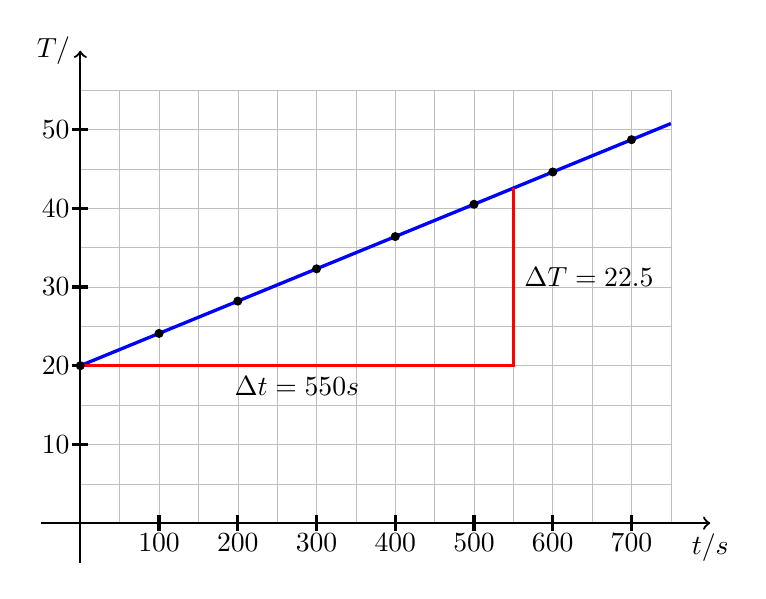
\begin{tikzpicture}[scale=1]
	\draw[style=help lines,step=0.5,gray!50] (0,0) grid (7.5,5.5);
	\draw [thick, ->] (-0.5,0) --(8,0) node[below]{$t/\text{s}$};
	\draw [thick, ->] (0,-0.5) --(0,6) node[left]{$T/\OC$};
	\foreach \s in {100,200,...,700}
	\draw [very thick] (\s/100,-0.1) -- (\s/100,0) node[below]{\s} -- (\s/100,0.1);
	\foreach \s in {10,20,...,50}
	\draw [very thick] (-0.1,\s/10) -- (0,\s/10) node[left]{\s} -- (0.1,\s/10);
	\draw [very thick,blue] (0,2) -- (7.5,5.075);
	\draw [very thick,red] (0,2) -- (5.5,2) node[midway,below]{\textcolor{black}{$\Delta t = 550 \text{ s}$}} -- (5.5,4.255) node[right,midway]{\textcolor{black}{$\Delta T = 22.5 \OC$}};
	\foreach \s in {0,1,...,7}
	\draw [fill] (\s,2+0.41*\s) circle(0.05);
	\end{tikzpicture}
\end{figure}

\sol energy supplied: $Q = cm\Delta T \RA IV\Delta t = cm\Delta T \RA c = \frac{IV}{m \tfrac{\Delta T}{\Delta t}} $

$\frac{\Delta T}{\Delta t}$ is gradient of fitting line: $\frac{\Delta T}{\Delta t} = \frac{22.5}{550} \approx 4.09 \times 10^{-2} \text{ } \OC \text{ s}^{-1}$

specific heat capacity: $c = \frac{4.2\times12}{1.00 \times 4.09 \times 10^{-2}} \approx 1230 \jpkgC$	\eoe

\question{A mixture contains 5\% silver and 95\% of gold by weight. Some gold is melted and the correct weight of silver is added. The initial temperature of silver is $20^\circ$C. Use the data to calculate the initial temperature of gold so that the final mixture is at melting point of gold.}

\begin{center}
	\begin{tabular}{|l|c|c|}
		\hline  & silver & gold \\ 
		\hline melting point (K) & 1240 & 1340 \\ 
		\hline specific heat capacity (solid or liquid) (J kg$^{-1}$ K$^{-1}$) & 235 & 129 \\ 
		\hline specific latent heat of fusion (kJ kg$^{-1}$) & 105 & 628 \\
		\hline 
	\end{tabular} 
\end{center}



\subsection{internal energy}

we now consider the total energy within a thermodynamic system

molecules in a system undergo random motion, so they have kinetic energy

there are potential energy between molecules due to intermolecular interaction

\begin{ilight}
	\keypoint{internal energy}\index{internal energy} is defined as the sum of random kinetic energy of molecules and potential energy between molecules: $\boxed{U=E_k+E_p}$
\end{ilight}

\cmt internal energy is a \emph{state function} of the system

it only depends on current state of system, not on process to arrive at this state

\subsection{kinetic energy}

\cmt internal energy counts K.E. due to random motion at molecular level

K.E. of macroscopic motion of the system as a whole is not included

\cmt mean K.E. of molecules is directly proportional to temperature: $\boxed{E_k \propto T}$

K.E. of molecules depends on temperature only

higher temperature means molecules move faster, vibrate more intensively, etc.





\subsection{potential energy}

\cmt internal energy counts P.E. due to force fields \emph{within} the system

P.E. of the system as a whole due to \emph{external} force fields is not included

\cmt P.E. between molecules depends on intermolecular separation and chemical bonding

in general, greater intermolecular separation means greater P.E.\footnote{Intermolecular separation does not necessarily increase during melting processes. A typical counter example is melting of ice into water, for which intermolecular separation actually decreases (density of water > density of ice), but potential energy of the system will still increase because hydrogen bonds between H$_2$O molecules are broken.}: $\boxed{r \up \Leftarrow E_p \up}$

breaking intermolecular bonds also causes an increase in P.E.

mean P.E. of gas $>$ mean P.E. of liquid $>$ mean P.E. of liquid solid

\subsection{internal energy of ideal gas}

for ideal gas, mean K.E. of one molecule: $E_k = \frac{3}{2}kT$

there is no intermolecular force, so P.E. of ideal gas is defined to be zero: $E_p = 0$

internal energy per molecule: $U = E_k + E_p = \frac{3}{2}kT$

hence internal energy of ideal gas is purely kinetic and directly proportional to temperature

total internal energy of the gas: $U_\text{gas} = NU \RA \boxed{U_\text{gas} = \frac{3}{2}NkT}$

\subsection{change of states}

consider a substance being heated from its solid state

it will melt into a liquid and further vaporise into its gaseous state

we now look into the changes of internal energy during each stage

\begin{figure}[ht]
\centering
\begin{tikzpicture}[scale=1]
\draw[thick,->] (-1,-2) -- (0,-2) -- (10,-2) node[below] {$t$};
\draw[thick,->] (0,-2.5) -- (0,5) node[left]{$T$};
\draw [very thick,blue] (0,-1) node[left]{$A$} -- (1,0) node[above]{$B$} -- (2.5,0) node[above left]{$C$} -- (4,3) node[above]{$D$} -- (9,3) node[above left]{$E$} -- (9.5,4.5) node[above]{$F$};
\draw[thick,dashed] (4,3) -- (0,3) node[left]{$T_\text{boiling}$};
\draw[thick,dashed] (1,0) -- (0,0) node[left]{$T_\text{melting}$};
\end{tikzpicture}
\end{figure}


\begin{compactitem}
\item[--] $AB$ (solid state): $T \up \ra E_k \up$, greater vibration for solid particles

but no (significant) change in mean separation\footnote{A typical solid material expands when it is heated, so intermolecular separation will increase slightly.} $\ra$ no change in P.E.

\item[--] $BC$ (\emph{melting}): latent heat goes into breaking intermolecular bonds, $r\up \ra E_p \up$

but melting occurs at constant temperature\footnote{Here we talk about \emph{pure substance}, which changes from solid into liquid at a particular temperature, called the \emph{melting point}. But for a \emph{mixture} of substances, melting may occur over a \emph{range} of temperatures. It is also possible for a substance to decompose before they change states.} $\ra$ no change in K.E.

\item[--] $CD$ (liquid state): $T \up \ra E_k \up$, greater vibration and free motion

but no (significant) change in mean separation $\ra$ no change in P.E.

\item[--] $DE$ (\emph{boiling}): molecules break free, $r\up \ra E_p \up$

boiling occurs at constant temperature\footnote{Again we only concern pure substances. Mixtures that boil over a range of temperatures or substance decompose before phase transition are not considered here.} $\ra$ no change in K.E.

\item[--] $EF$ (gas state): $T \up \ra E_k \up$ particles move even faster

particles completely separated, no intermolecular force, so constant $E_p = 0$
\end{compactitem}

\question{For a particular substance, why is the specific latent heat of vaporisation much greater than the specific latent heat of fusion?}

\subsection*{evaporation}

liquid changes into gas without boiling $\longrightarrow$ \keypoint{evaporation}

particles move randomly, i.e., they move at various speeds

some molecules move fast enough to break free

\cmt \emph{cooling effect}: evaporation causes a decrease in temperature of the liquid

most energetic molecules escaped, those remain in the liquid have less energy, $E_k \down \ra T \down$

\cmt rate of evaporation increases with temperature, surface area of liquid

\cmt different between boiling and evaporation

\begin{center}
	\begin{tabular}{|c|c|c|}
		\hline 
		& boiling & evaporation \\ 
		\hline 
		occurrence & throughout the liquid & at surface only \\ 
		\hline 
		temperature & occur at boiling point & occur at any temperature \\ 
		\hline 
		bubble formation & bubbles formed & no bubbles \\ 
		\hline 
		rate of process & fast & slow \\ 
		\hline 
	\end{tabular} 
\end{center}

\subsection{first law of thermodynamics}

internal energy of a system changes upon heat transfer or doing work

\begin{ilight}
	\keypoint{first law of thermodynamics}\index{law of thermodynamics!first law of thermodynamics} states that the increase in internal energy equals sum of heat supply to the system and work done on the system: $\boxed{\Delta U = Q +  W}$
\end{ilight}

\cmt first law of thermodynamics is an extension of the law of conservation of energy

\cmt sign conventions for $Q$ and $W$

\begin{compactitem}
	\item[$\circ$] $Q>0$ if heat supplied to system
	
	\item[$\circ$] $Q<0$ if heat released by system to surroundings
	
	\item[$\circ$] $W>0$ if work done \emph{on} system by external
	
	i.e., if system is compressed and volume decreases, then $W>0$
	
	\item[$\circ$] $W<0$ if system does work \emph{against} surroundings
	
	i.e., system expands and volume increases, then $W<0$
	
\end{compactitem}

\cmt amount of heat energy: $Q=\left\{ \begin{array}{l}
	cm\Delta T \qquad (\text{if no change of state}) \\
	Lm \qquad (\text{during change of state})
	\end{array}\right.$

\cmt amount of work is related to pressure and change of volume

if volume changed at \emph{constant} pressure, then $W=F\Delta s = pA\Delta s \ra \boxed{W = p\Delta V}$\footnote{If pressure changes with volume during a thermodynamics process, then work done $W=\int p \dd V$. Alternatively, we can evaluate the area under a $p$-$V$ graph to find the work done.}

if no change of volume, then no work is done

\begin{figure}[h]
		\begin{tikzpicture}[domain=1:9]
		\draw[->] (-0.5,0) -- (12,0) node[anchor=north] {$V$};
		\draw[->] (0,-0.5) -- (0,10) node[anchor=east] {$P$};
		\draw (1,9) node[anchor=south]  {\textbf{A}};
		\draw[thick, ->]  (1,9) .. controls (4,7) and (7,6.2) .. (8,6) node[midway, anchor=south west] {\textbf{1}};
		\draw[thick, ->] (8,6) .. controls (9,4.5) and (10,3) .. (12,1) node[anchor=south west, midway] {\textbf{2}};
		\draw[thick, ->] (12,1) .. controls (8,1.5)  .. (3,3) node[midway, anchor=north east] {\textbf{3}};
		\draw[thick, ->] (3,3) .. controls (1.6,6)  .. (1,9) node[midway, anchor=north east] {\textbf{4}};
		\end{tikzpicture}
		\caption{The Carnot Cycle}
		\label{carnotcycle}
	\end{figure}
 
The Carnot Cycle shown in Figure \ref{carnotcycle} is commonly used to test the understanding for the first law. The cycle begins and ends at point \textbf{A}. This means that the internal energy of the system at the start and end of the cycle is the same (as $PV=nRT$ and $T$ is proportional to the internal energy). The changes at each stage of the cycle are as follows:
	
	\begin{description}
		\item[1. Isothermal Expansion] In stage 1 the gas expands at contant temperature. Since it is expanding, the gas is doing work on the surroundings and since it is at constant temperature the internal energy of the gas remains constant. Therefore the second law implies that the gas must be absorbing heat. \emph{Note that isothermal changes are often indicated by describing the change as occuring slowly.}
		\item[2. Adiabatic Expansion] In stage 2 the gas expands without transferring heat to/from the surroundings. Since it is doing work the gas's internal energy drops, as does its temperature.
		\item[3. Isothermal Compression] In stage 3 the gas is compressed at constant temperature. Since work is done on the gas and the internal energy remains constant it must be the case that heat is lost to the surroundings.
		\item[4. Adiabatic Compression] Finally, the gas is compressed without heat transfer to/from the surroundings. Work is done on the gas and therefore the internal energy, and termperature, increase.
	\end{description}
	
	
	\begin{example}
		
		Complete the table for the Carnot Cycle shown in figure \ref{carnotcycle}.
		
		\begin{tabular}{|c|p{3cm}|p{3cm}|p{3cm}|}
			\hline
			stage & \centering thermal energy supplied \textbf{to} the gas / J & \centering work done \textbf{on} the gas / J & \centering \textbf{increase} in internal energy of the gas / J \tabularnewline \hline
			1 & \centering\centering(a) & \centering-936 & \centering(b) \tabularnewline \hline
			2 & \centering0 & \centering(c) & \centering(d) \tabularnewline \hline
			3 & \centering(e) & \centering+702 & \centering0 \tabularnewline \hline
			4 & \centering(f) & \centering+844 & \centering+844 \tabularnewline \hline
		\end{tabular}
		
		
		
		In stage 1 there is no change in internal energy of the gas, so (b) equals zero. In order to satisfy the first law of thermodynamics the thermal energy supplied must equal the work done \textbf{by} the gas so (a) equals +936J.
		
		As the total change in internal energy throughout the cycle must be zero, we can now calculate (d) as being -844J.
		
		(c) can be calculated using the first law as -844J.
		
		A similar argument to that used in stage 1 can be used in stage 3 to give (e) as -702J.
		
		In stage 4 no energy is transferred by heating therefore (f) is equal to zero.
		
		
		
		The final table is therefore:
		
		\begin{tabular}{|c|p{3cm}|p{3cm}|p{3cm}|}
			\hline
			stage & \centering thermal energy supplied \textbf{to} the gas / J & \centering work done \textbf{on} the gas / J & \centering \textbf{increase} in internal energy of the gas / J \tabularnewline \hline
			1 & \centering\centering \textbf{+936} & \centering-936 & \centering \textbf{0} \tabularnewline \hline
			2 & \centering0 & \centering \textbf{-844} & \centering \textbf{-844} \tabularnewline \hline
			3 & \centering \textbf{-702} & \centering+702 & \centering0 \tabularnewline \hline
			4 & \centering \textbf{0} & \centering+844 & \centering+844 \tabularnewline \hline
		\end{tabular}
		
	\end{example} 

\example{A gas is heated by supplying it with 25 kJ of energy. The gas expands so that the volume increases by 0.10 m$^3$. Assume the gas has a fixed pressure of 150 kPa during the process. Calculate the change in internal energy.}

\sol amount of work done: $W = p \Delta V = 150 \times 0.10 = 15 \text{ kJ}$

but gas expands means work is done against surroundings, so this is negative work

change in internal energy: $\Delta U = Q +  W = (+25) + (-15) = +10 \text{ kJ}$ \eoe

\example{Use the idea of internal energy and the first law of thermodynamics, explain why boiling water requires heat supply.}

\sol boiling occurs at constant temperature, so $\Delta E_k = 0$

but separation between molecules increased, so $\Delta E_p >0$

by definition, internal energy $U=E_k+E_p$, so $\Delta U >0$

during boiling, there is an increase in volume, so work against surroundings, $W<0$

recall first law of thermodynamics $\Delta U = Q + W$, must have $Q>0$

this means heat must be supplied for boiling processes \eoe

\example{When you pump up a bicycle tyre, the temperature of air inside the tyre will go up. Explain why this happens using the first law of thermodynamics.}

\sol pumping up tyre involves compressing gas, so positive work is done: $W>0$

for each stroke, there is little time for heat transfer, so $Q \approx 0$

according to first law of thermodynamics $\Delta U = Q + W \RA \Delta U >0$

by definition, internal energy $U=E_k + E_p \RA \Delta U = \Delta E_k + \Delta E_p>0$

but for gas, there is negligible intermolecular force, so $\Delta E_p=0$, then must have $\Delta E_k>0$

K.E. of molecules is proportional to temperature, higher K.E. so higher temperature \eoe

\example{An ideal gas of 0.080 mol is initially at state $A$ and then undergoes a cycle $ABCA$. The variation of its pressure $p$ with its volume $V$ is shown on the graph.}

\begin{figure}[ht]
	\centering
	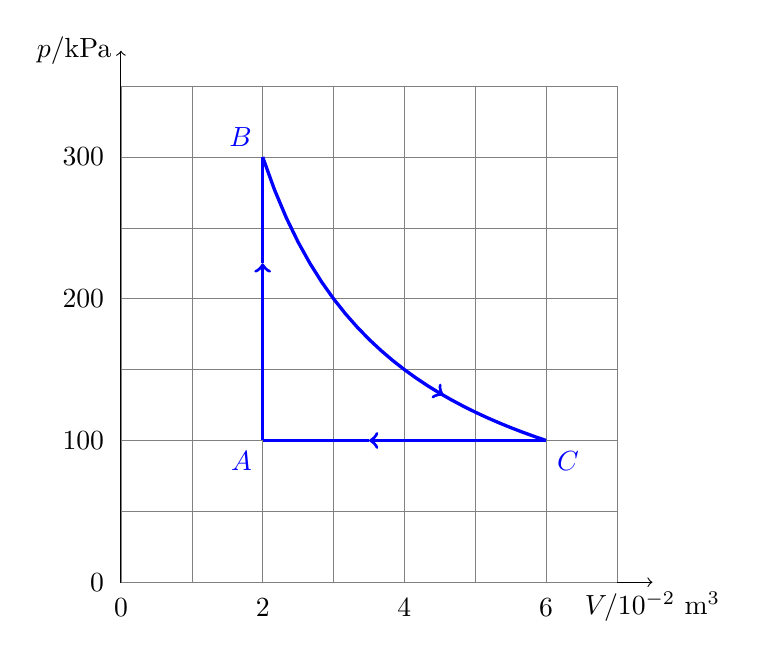
\begin{tikzpicture}[scale=0.9]
	\draw[<->] (0,7.5) node[left]{$p$/kPa} -- (0,0) -- (7.5,0) node[below] {$V/10^{-2}$ m$^3$};
	\draw[help lines, gray] (0,0) grid (7,7);
	\foreach \x in {0,100,200,300} \node[left] at (-0.1,\x*2/100) {$\x$};
	\foreach \x in {0,2,4,6} \node[below] at (\x,-0.1) {$\x$};
	\draw[very thick, blue, ->] (2,2) node[below left]{$A$} -- (2,4.5);
	\draw[very thick, blue] (2,4.5) -- (2,6) node[above left]{$B$};
	\draw [very thick, blue, domain=2:6] plot (\x, {12/\x}) node[below right]{$C$};
	\draw[very thick, blue, ->] (6,2) -- (3.5,2);
	\draw[very thick, blue] (3.5,2) -- (2,2);
	\draw[very thick, blue, ->] (4.5,2.67) -- (4.55,2.64);
	\end{tikzpicture}
\end{figure}

Temperature of state $A$ is 300 K. The magnitude of work on gas from state $B$ to $C$ is 6570 J.

For each stage $A \to B$, $B \to C$ and $C \to A$ during the cycle, determine work done and heat supply to the gas, and also find the change in internal energy.

\newpage

\sol work done depends on change in volume

$A\to B$: no change in volume, so $W_{AB} = 0$

$B \to C$: $|W_{BC}|= 6570 \text{ J}$, but expansion implies $W<0$, so $W_{BC}=-6570 \text{ J}$

$C \to A$: $|W_{CA}| = p\Delta V_{CA} = 1\times10^5 \times (6-2)\times10^{-2} \RA W_{CA}= +4000 \text{ J}$ (compression so $W>0$)

\noindent change in internal energy of ideal gas depends on change in temperature

$A\to B$: same $V$ but $p_B = 3p_A$, so $T_B = 3T_A = 900 \text{ K}$

$\phantom{A\to B\text{: }}\Delta U_{AB} = \frac{3}{2}Nk\Delta T_{AB} = \frac{3}{2}\times 0.80\times 6.02\times10^{23}\times1.38\times10^{-23}\times(900-300) \approx +5980 \text{ J}$

$B \to C$: note that $p_BV_B = p_CV_C$, so $T_B = T_C$, no change in temperature, so $\Delta U_{BC}=0$

$C \to A$: $\Delta U_{CA} = \frac{3}{2}Nk\Delta T_{CA} = \frac{3}{2}\times 0.80\times 6.02\times10^{23}\times1.38\times10^{-23}\times(300-900) \approx -5980 \text{ J}$


for cycle $ABCA$, same initial and final state, so total change in internal energy must be zero

one can check that $\Delta U_\text{cycle} = \Delta U_{AB} + \Delta U_{BC} + \Delta U_{CA} = 0$
	
\noindent to find supply of thermal energy, we apply first law of thermodynamics: $\Delta U = Q + W$

$A\to B$: $+5980 = Q_{AB} + 0 \RA Q_{AB} = +5980 \text{ J}$

$B \to C$: $0 = Q_{BC} + (-6570) \RA Q_{BC} = +6570 \text{ J}$

$C \to A$: $-5980 = Q_{CA} + (+4000) \RA Q_{CA} = -9980 \text{ J}$

\noindent the table below summarises all energy changes during the cycle $ABCA$
\begin{center}
		\begin{tabular}{|C{2.5cm}|C{2.5cm}|C{2.5cm}|C{2.5cm}|}
			\hline
			change &  $W$/J & $Q$/J & $\Delta U$/J \\ \hline
			$A \to B$ & 0 & +5980 & +5980\\ \hline
			$B \to C$ & -6570 & +6570 & 0 \\ \hline
			$C \to A$ & +4000 & -9980 & -5980 \\ \hline
		\end{tabular}
	
	\vspace*{-0.1\baselineskip}\eoe
\end{center}

\question{Show that when $n$ mol of gas is heated at a fixed volume, thermal energy required to raise the temperature by 1.0 K is $nR$.}

\question{Two identical balloons $A$ and $B$ hold the same amount of gas at the same initial temperature. They are given the same amount of heat. Suppose volume of $A$ is fixed, while $B$ is allowed to expand, compare the final temperatures of the gases in the two balloons.}


\subsection{temperature}

\subsection{temperature \& thermal energy}

\cmt temperature can be considered as a \emph{relative} measure of thermal energy

temperature can tell the \emph{direction} of thermal energy flow

heat always (spontaneously) flows from high temperature regions to colder regions\footnote{This is the consequence of the \emph{second law of thermodynamics}\index{law of thermodynamics!second law of thermodynamics \piste}, which is concerned with the direction of natural processes. The law states that the total \emph{entropy}, a quantity that counts the number of microstates of a system, of an isolated system can never decrease over time. You will learn more about entropy if you study A-Level chemistry.}

\cmt if two objects in contact have the same temperature, then there is no net heat transfer

the two objects are said to be in \keypoint{thermal equilibrium}\index{thermal equilibrium}

\cmt if two systems $A$ and $B$ are each in thermal equilibrium with a third system $C$, $A$ and $B$ are also in thermal equilibrium, this is called the \keypoint{zeroth law of thermodynamics}\index{law of thermodynamics!zeroth law of thermodynamics}
\footnote{This law is important for the formulation of thermal physics. The physical meaning of the law was expressed by Maxwell: "All heat is of the same kind." The zeroth law allows us to give the mathematical definition of temperature.}

\question{A student thinks that temperature measures the amount of heat in an object. Suggest why this statement is incorrect with examples.}

\subsection{absolute zero}\label{s-abs-zero}

mean K.E. of molecules is a microscopic description of temperature $T$

minimum K.E. occurs if molecules do not move at all (completely frozen)\footnote{In the \emph{classical} description, there is no reason not allowing a molecule to cease motion. However, due to \emph{quantum mechanical effects}, kinetic energy of a system cannot be zero even at absolute zero.}

this corresponds to the lowest possible temperature, called \keypoint{absolute zero}\index{absolute zero}

\cmt \keypoint{Kelvin scale of thermodynamic temperature} is defined based on absolute zero as 0 K\footnote{More precisely, 0 K for absolute zero  and $273.16\text{ K}$ for water triple point.}

\cmt conversion rule between Celsius scale and Kelvin scale: $\boxed{T_K (\text{K}) \text{ } \autorightleftharpoons{\footnotesize -273.15}{\footnotesize +273.15} \text{ } T_C (\OC)}$\footnote{The numerical value of 273.15 will only be quoted in this chapter. For everywhere else in the notes, we will use the less precise value 273 for simplicity.}

\cmt Kelvin scale is said to be an \emph{absolute scale}

zero of Kelvin scale does not depend on property of a specific substance

in contrast, zero of Celsius scale is based on properties of water

\cmt it is impossible to remove any more energy from a system at 0 K (or -273.15 \OC)

but there is no practicable means to bring a physical system to exactly $0\text{ K}$
\footnote{This is known as the \emph{third law of thermodynamics}\index{law of thermodynamics!third law of thermodynamics \piste}, which states that it is impossible, no matter how idealized, to reduce the temperature of any closed system to absolute zero in a finite number of operations.}




\subsection{thermometer}

a \keypoint{thermometer}\index{thermometer} is a device which can be used to measure temperature



\subsection*{liquid-in-glass thermometer}

basic principle: liquid expands in volume at higher temperature

examples include alcohol thermometer, mercury-in-glass thermometer, etc.

\begin{center}
	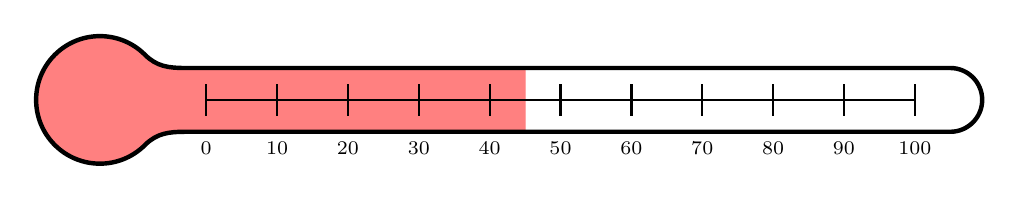
\begin{tikzpicture}[scale=1.35]
		\draw[red!50,fill] (45:0.6) arc(45:315:0.6) [out=45, in=180] to (0.8,-0.3) -- (4,-0.3) -- (4,0.3) -- (0.8,0.3) [out=180, in=-45] to (45:0.6);
		\draw[ultra thick] (45:0.6) arc(45:315:0.6) [out=45, in=180] to (0.8,-0.3) -- (8,-0.3) arc(-90:90:0.3) -- (0.8,0.3) [out=180, in=-45] to (45:0.6);
		\draw[thick] (1,0) -- (7.67,0);
		\foreach \temp in {0,10,20,...,100}{
			\draw[thick] (1+\temp/15,-0.15) --++ (0,0.3);
			\node[below] at (1+\temp/15,-0.3) {{\scriptsize \temp\OC}};
		}
	\end{tikzpicture}
\end{center}

\subsection*{resistance temperature detectors (RTD)}

basic principle: resistance of electronic element changes with temperature

metal wires and thermistor are both used in RTD elements 


\subsection*{thermocouple}\index{thermocouple}

basic principle: difference in temperature can produce a \emph{thermoelectric voltage} across junctions, thermocouple measures temperatures by means of this voltage

\begin{figure}[ht]
	\centering
	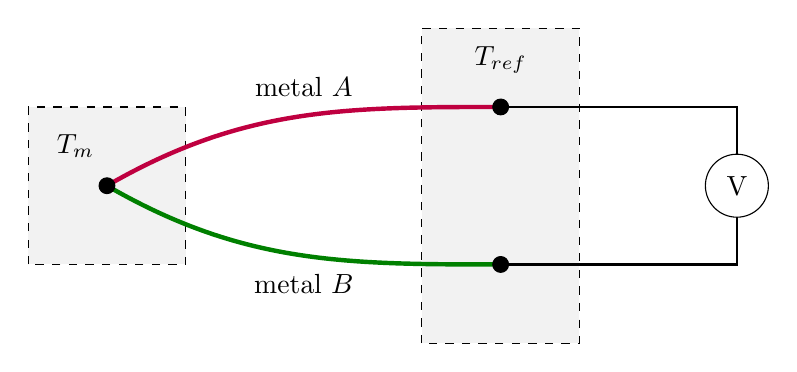
\begin{tikzpicture}
		% temp region boxes
		\draw[dashed,fill=gray!10] (-6,-1) rectangle (-4,1);
		\node at (-5.4,0.5) {$T_m$};
		\draw[dashed,fill=gray!10] (-1,-2) rectangle (1,2);
		\node at (0,1.6) {$T_\text{ref}$};
		% wires and junctions
		\draw[ultra thick,purple] (-5,0) [out=30,in=180] to (0,1);
		\node at (-2.5,1.25) {metal $A$};
		\node at (-2.5,-1.25) {metal $B$};
		\draw[ultra thick,Green] (-5,0) [out=-30,in=180] to (0,-1);
		\draw[fill] (-5,0) circle(0.1);
		\draw[fill] (0,1) circle(0.1);
		\draw[fill] (0,-1) circle(0.1);
		% connection to voltmeter
		\draw[thick] (0,1) --++ (3,0) --++ (0,-2) -- (0,-1);
		\draw[fill=white] (3,0) circle(0.4) node {V};
	\end{tikzpicture}
	
	\caption*{typical configuration of a thermocouple unit}
\end{figure}

two pieces of different metal wires are joined at their ends

if there exists a temperature difference between the ends, a \emph{thermoelectric voltage} is developed

this voltage depends on temperature difference, captured by some characteristic function

in practice, we place the \emph{measurement} junction in an environment of unknown temperature

the other end, or the \emph{reference} junction, is at a known temperature

temperature difference is deduced from the voltage reading

hence the desired temperature can be determined

\vspace*{\baselineskip}

\cmt features of a thermometer:
\begin{compactitem}
	\item[--] \emph{range}: whether the thermometer can measure very low or very high temperatures
	
	\item[--] \emph{sensitivity}: whether a small change in temperature can be detected
	
	\item[--] \emph{response time}: whether changes in temperature can be immediately measured
	
	\item[--] \emph{linearity}: whether changes in temperature are proportional to changes in output
	
\end{compactitem}

%\cmt any thermometer requires \emph{calibration}
%
%device must be checked and adjusted so that measurements are accurate

\begin{center}
	\begin{tabular}{|l|C{2.4cm}|C{2.4cm}|C{2.4cm}|C{2.4cm}|}
		\hline 
		& liquid-in-glass & RTD wire & thermistor & thermocouple \\ 
		\hline 
		valid range & narrow & wide & narrow & very wide \\ 
		\hline 
		sensitivity & low & fair & high & high \\ 
		\hline 
		response time & slow & fast & fast & very fast \\ 
		\hline 
		linearity & good & good & limited & non-linear \\ 
		\hline 
	\end{tabular} 
\end{center}


